% +------------------------------------------------------------------------+
% | CGAL User Manual: 
% +------------------------------------------------------------------------+
% |
% | 05.04.2004   Peter Hachenberger
% | 
\RCSdef{\NefpolyhedronRev}{$Revision$}
\RCSdefDate{\NefpolyhedronDate}{$Date$}
% +------------------------------------------------------------------------+

\ccParDims

\chapter{3D Nef Polyhedron}
\label{chapterNef_3}
\ccChapterRelease{\NefpolyhedronRev. \ \NefpolyhedronDate}\\
\ccChapterAuthor{Peter Hachenberger and Lutz Kettner}


\begin{lcTexBlock}
  \catcode`@=11
  \gdef\pyr{\mathop{\operator@font Pyr}\nolimits}
  \gdef\aff{\mathop{\operator@font aff}\nolimits}
  \catcode`@=12
\end{lcTexBlock}
\lcHtml{
  \newcommand{\pyr}{Pyr}
  \newcommand{\aff}{aff}
}

\minitoc

% +------------------------------------------------------------------------+
\section{Introduction}

\begin{ccTexOnly}
    \vspace*{-20mm}
    \begin{flushright}
      \parbox{0.3\textwidth}{%
          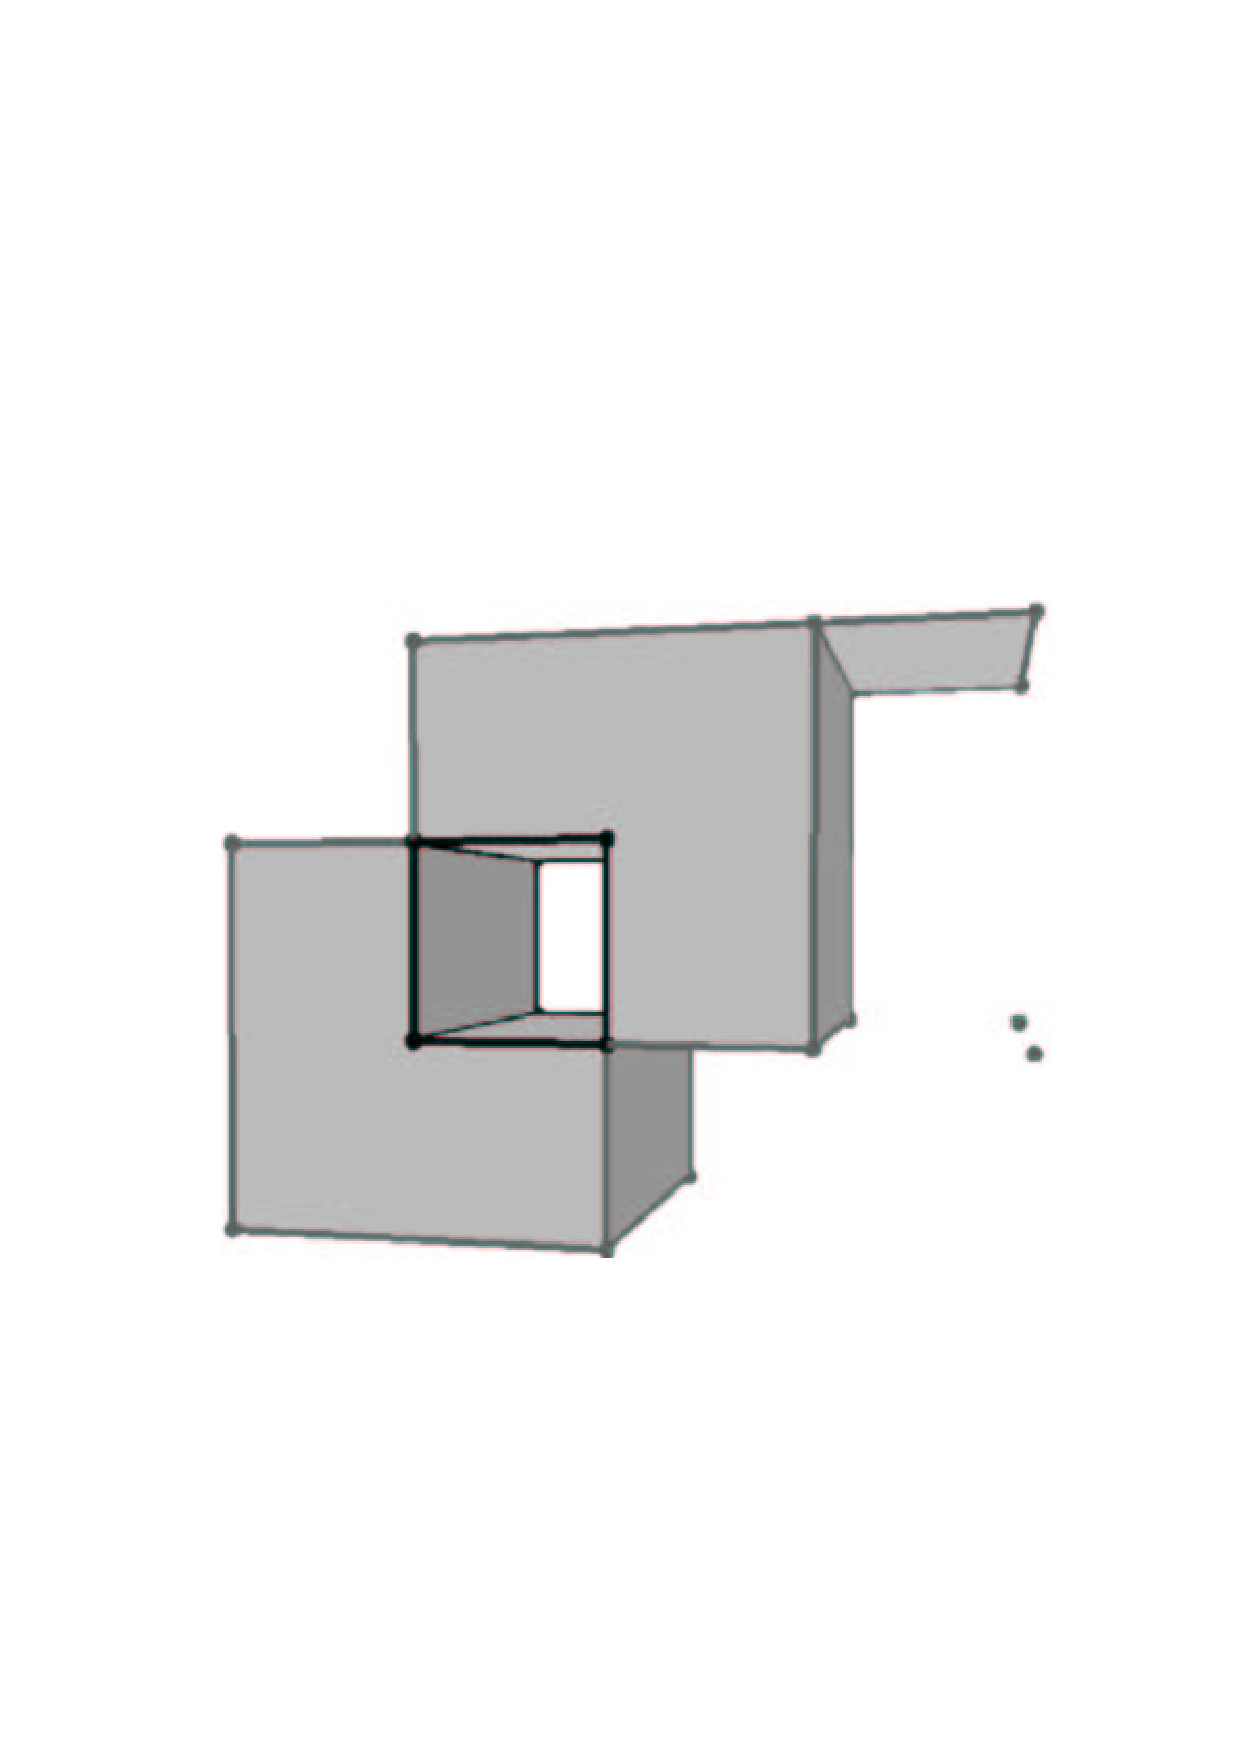
\includegraphics[width=0.3\textwidth]{Nef_3/fig/nef_non_manifold3a}%
      }%
    \end{flushright}
\end{ccTexOnly}

In solid modeling, two major representation schemes are used:
\emph{constructive solid geometry} (CSG) and \emph{boundary
  representations} (B-rep). Both have inherent strengths and
weaknesses, see \ref{cgal:h-gsmi-89} for a discussion.

In CSG a solid is represented as a set-theoretic boolean combination
of primitive solid objects, such as blocks, prisms, cylinders, or
toruses.  The boolean operations are not evaluated, instead, objects
are represented implicitly with a tree structure; leaves represent
primitive objects and interior nodes represent boolean operations or
rigid motions, e.g., translation and rotation. Algorithms on such a
CSG-tree first evaluate properties on the primitive objects and
propagate the results using the tree structure.
 
A B-rep describes the incidence structure and the geometric properties
of all lower-dimensional features of the boundary of a solid. Surfaces
are oriented to decide between the interior and exterior of a solid.

The class of representable objects in a CSG is usually limited by the
choice of the primitive solids. A B-rep is usually limited by the
choice for the geometry of the supporting curves for edges and the
supporting surfaces for surface patches, and, in addition, the
connectivity structure that is allowed. In particular, a B-rep is not
always closed under boolean set operations.  As an example, the class
of orientable 2-manifold objects is a popular and well understood
class of surfaces commonly used for B-reps. They can be represented
and manipulated efficiently, the data structures are compact in
storage size, and many algorithms are simple. On the other side, this
object class is not closed under boolean set operations, as many
examples can illustrate, such as the Figure shown above that can be
generated using boolean set operations on cubes. The vertices bounding
the tunnel, or the edge connecting the ``roof'' with the cube are
non-manifold situations.

In our implementation of Nef polyhedra in 3D, we offer a B-rep data
structure that is closed under boolean operations and with all their
generality. Starting from halfspaces (and also directly from oriented
2-manifolds), we can work with set union, set intersection, set
difference, set complement, interior, exterior, boundary, closure, and
regularization operations. In essence, we can evaluate a CSG-tree with
halfspaces as primitives and convert it into a B-rep representation.

In fact, we work with two data structures; one that represents the
local neighborhoods of vertices, which is in itself already a complete
description, and a data structure that connects these neighborhoods up
to a global data structure with edges, facets, and volumes. We offer a
rich interface to investigate these data structures, their different
elements and their connectivity. We provide affine (rigid)
transformations and a point location query operation. We have a custom
file format for storing and reading Nef polyhedra from files. We offer
a simple OpenGL-based visualizer for debugging and illustrations.


% +------------------------------------------------------------------------+
\section{Definition}

The theory of Nef polyhedra has been developed for arbitrary
dimensions. The class \ccc{CGAL::Nef_polyhedron_3} implements a
boundary representation for the 3-dimensional case.

\vspace{2ex}{\bf Definition:}\quad
    A \emph{Nef-poly\-he\-dron} in dimension $d$ is a point set $P \subseteq
    \R^d$ generated from a finite number of open halfspaces by set
    complement and set intersection operations.
\vspace{2ex}

Set union, difference and symmetric difference can be reduced to
intersection and complement. Set complement changes between open
and closed halfspaces, thus the topological operations \emph{boundary},
\emph{interior}, \emph{exterior}, \emph{closure} and {\em
regularization} are also in the modeling space of Nef polyhedra.

A face of a Nef polyhedron is defined as an equivalence class of
\emph{local pyramids} that are a characterization of the local space
around a point.

\vspace{2ex}{\bf Definition:}\quad
    A point set $K \subseteq \R^d$ is called a \emph{cone with apex $0$},
    if $K = \R^{+} K$ (i.e., $\forall p \in K, \forall \lambda > 0: \lambda p
    \in K$) and it is called a \emph{cone with apex $x$}, $x \in \R^d$,
    if $K = x + \R^{+} (K - x)$. A cone $K$ is called a \emph{pyramid}
    if $K$ is a polyhedron.

    Now let $P \in \R^d$ be a polyhedron and $x \in \R^d$. There is a 
    neighborhood $U_0(x)$ of $x$ such that the pyramid $Q := x + \R^{+} 
    ((P \cap U(x)) - x)$ is the same for all neighborhoods $U(x) \subseteq
    U_0(x)$. $Q$ is called the \emph{local pyramid} of $P$ in $x$ and
    denoted $\pyr_P(x)$. 
\vspace{2ex}

{\bf Definition:}\quad
    Let $P \in \R^d$ be a polyhedron and $x, y \in \R^d$ be two points.
    We define an equivalence relation $x \sim y$ iff
    $\pyr_P(x) = \pyr_P(y)$. The equivalence classes of $\sim$ 
    are the \emph{faces} of $P$. The dimension of a face $s$ is the  
    dimension of its affine hull, $\dim s := \dim \aff s$.
\vspace{2ex}

In other words, a \emph{face} $s$ of $P$ is a maximal non-empty subset
of $\R^d$ such that all of its points have the same local pyramid $Q$
denoted $\pyr_P(s)$.  This definition of a face partitions $\R^d$ into
faces of different dimension. A face $s$ is either a subset of $P$, or
disjoint from $P$.  We use this later in our data structure and store
a selection mark in each face indicating its set membership.

Faces do not have to be connected. There are only two full-dimensional
faces possible, one whose local pyramid is the space $\R^d$ itself and
the other with the empty set as a local pyramid.
All lower-dimensional faces form the \emph{boundary} of
the polyhedron. As usual, we call zero-dimensional faces {\em
vertices} and one-dimensional faces \emph{edges}. In the case of
polyhedra in space we call two-dimensional faces \emph{facets} and
the full-dimensional faces \emph{volumes}. Faces are \emph{relative
open} sets, e.g., an edge does not contain its end-vertices.

    We illustrate the definitions with an example in the plane.
    Given the closed halfspaces
    \[\begin{array}{lllll}
        h_1: y \ge 0,\ \ \    &
        h_2: x - y \ge 0,\ \ \ &
        h_3: x + y \le 3,\ \ \ &
        h_4: x - y \ge 1,\ \ \ &
        h_5: x + y \le 2, 
      \end{array}
    \]
    we define our polyhedron $P := ( h_1 \cap h_2 \cap h_3) - ( h_4 \cap h_5)$.

\begin{minipage}[t]{0.5\textwidth}
\begin{ccTexOnly}
    \begin{center}
      \parbox{0.7\textwidth}{%
          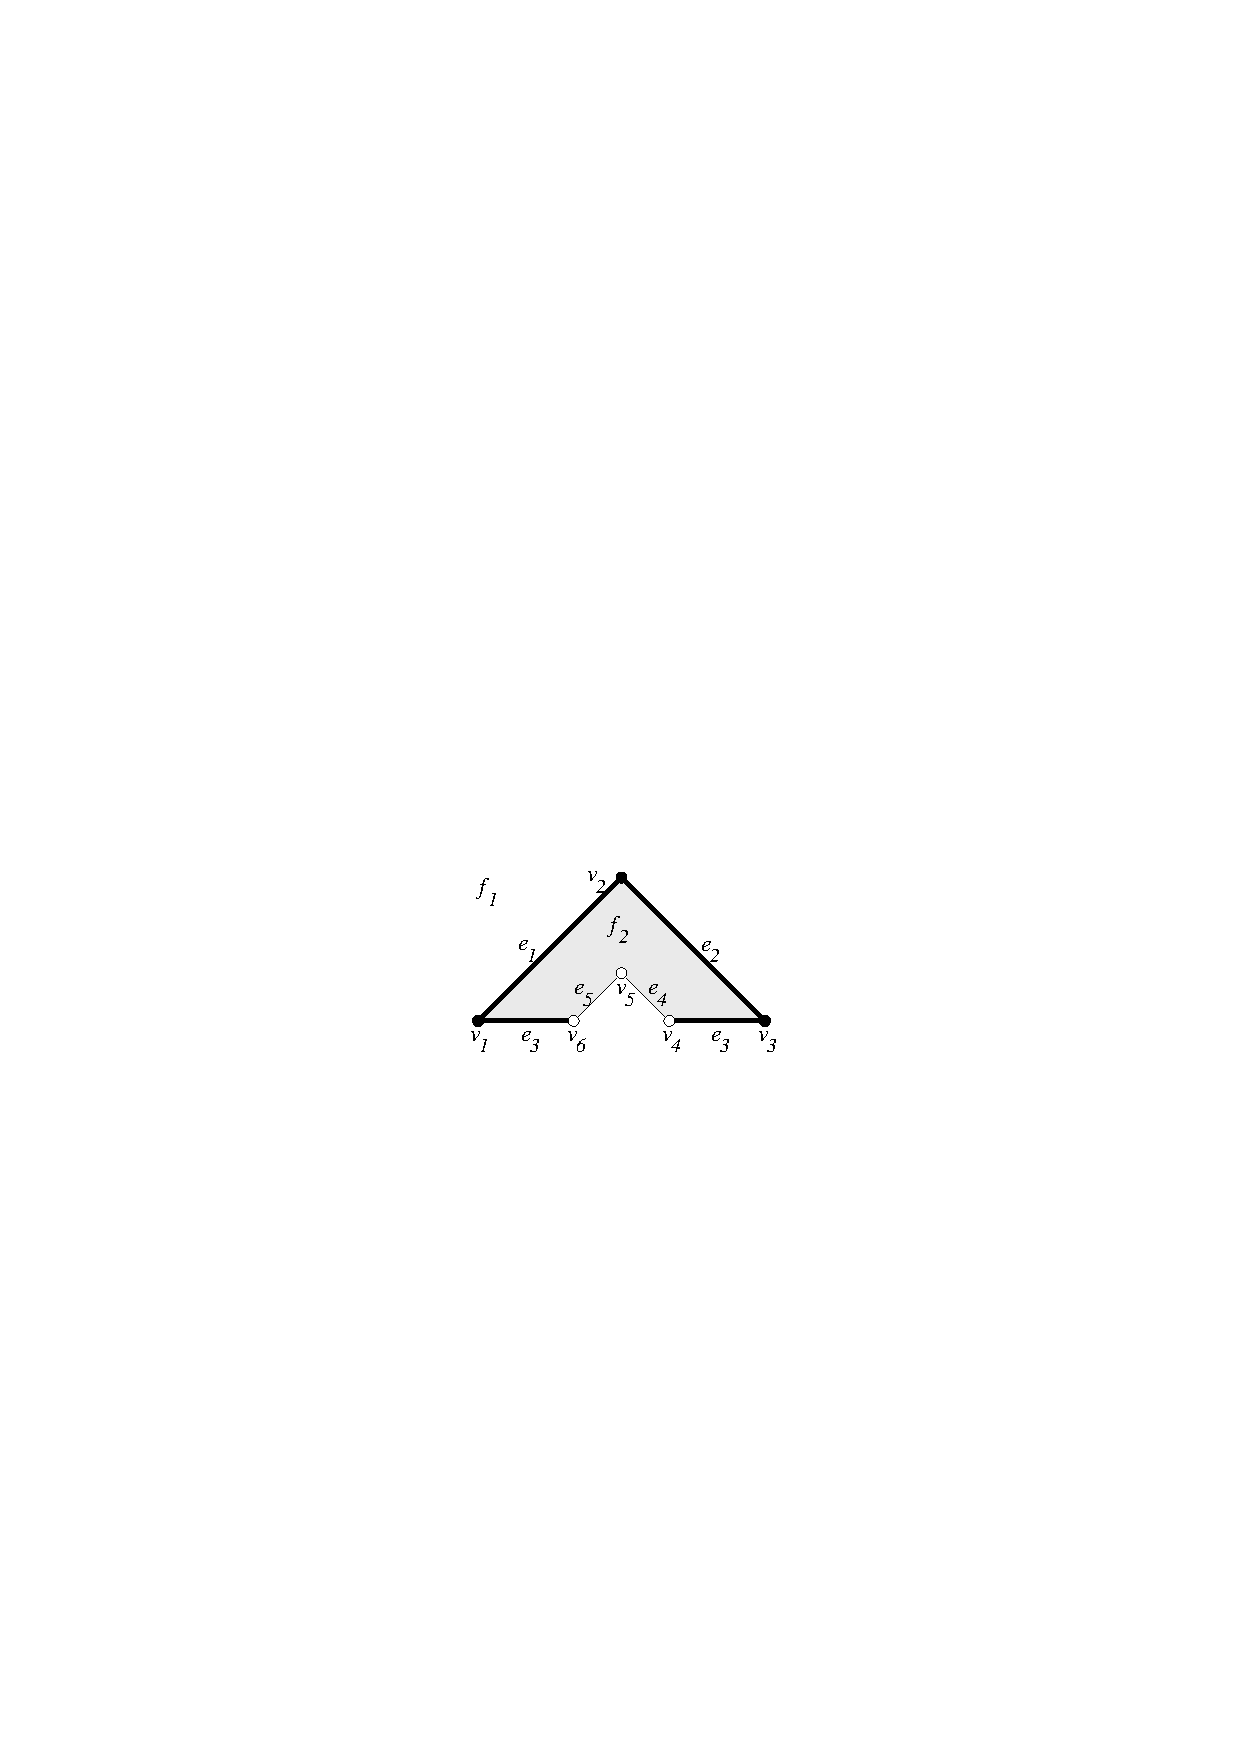
\includegraphics[width=0.70\textwidth]{Nef_3/fig/nef_example}%
      }
    \end{center}
\end{ccTexOnly}

\begin{ccHtmlOnly}
    <CENTER>
        <img src="fig/nef_example.gif" alt="Steps in making a cube."><P>
    </CENTER>
\end{ccHtmlOnly}
\end{minipage}
\begin{minipage}[t]{0.5\textwidth}
\begin{ccTexOnly}
    \begin{center}
      \parbox{0.8\textwidth}{%
          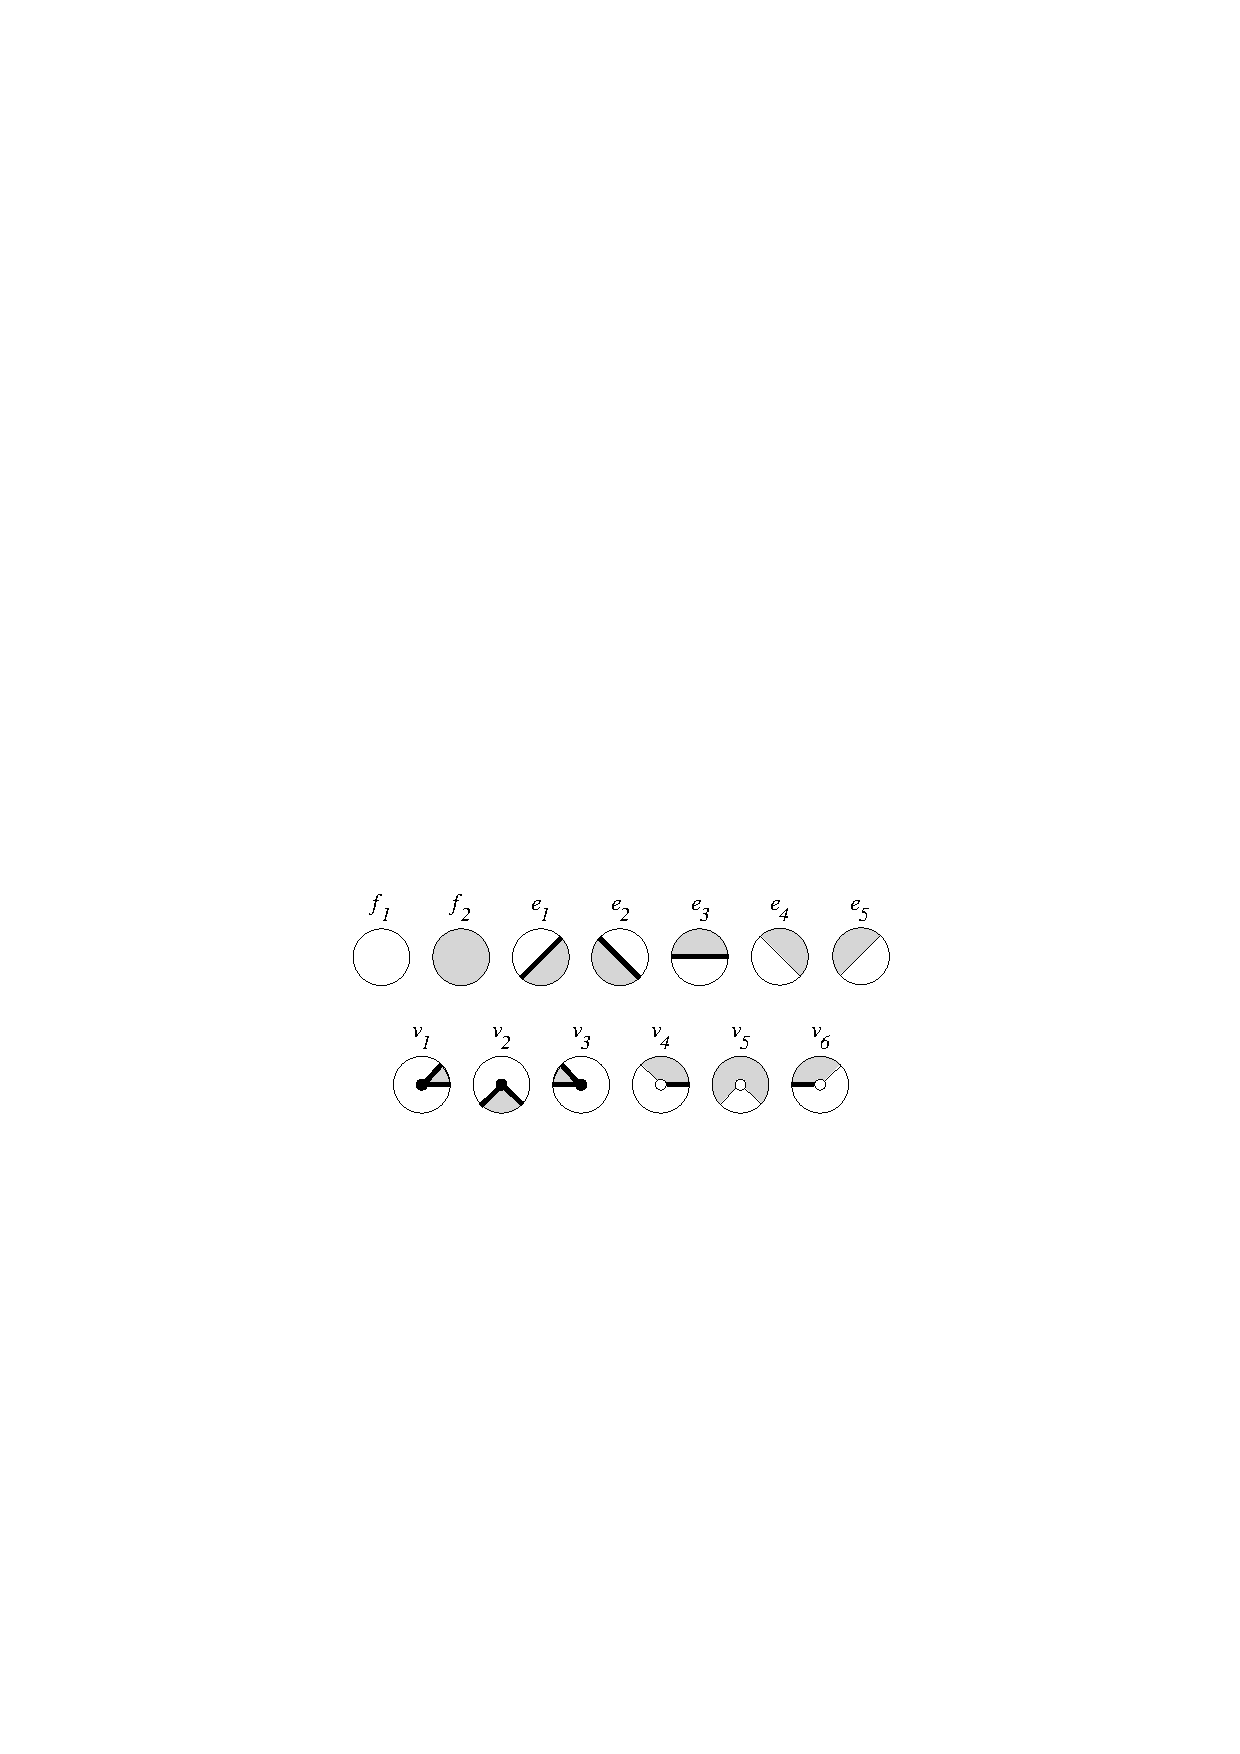
\includegraphics[width=0.80\textwidth]{Nef_3/fig/nef_pyramids}%
      }
    \end{center}
\end{ccTexOnly}

\begin{ccHtmlOnly}
    <CENTER>
        <img src="fig/nef_pyramids.gif" alt="Steps in making a cube."><P>
    </CENTER>
\end{ccHtmlOnly}
\end{minipage}

The left figure illustrates the polyhedron with
its partially closed and partially open boundary, i.e., vertex 
$v_4, v_5, v_6$, and edges $e_4$ and $e_5$ are not part of $P$.
The local pyramids for the faces are $\pyr_P(f_1) = \emptyset$
and $\pyr_P(f_2) = \R^2$. Examples for the local pyramids of edges
are the closed halfspace $h_2$ for the edge $e_1$, $\pyr_P(e_1) = h_2$,
and the open halfspace that is the complement of $h_4$ for the 
edge $e_5$, $\pyr_P(e_5) =
\{(x,y) | x - y < 1\}$. The edge $e_3$ consists actually of two
disconnected parts, both with the same local pyramid $\pyr_P(e_3) = h_1$.
In our data structure, we will represent the two connected
components of the edge $e_3$ separately.
The figure on the right  
lists all local pyramids for this example.


The local pyramids of each vertex are represented by
conceptually intersecting the local neighborhood with a small
$\varepsilon$-sphere. This intersection forms a planar map on the
sphere (see figure below), which together with the set-selection
mark for each item forms a two-dimensional Nef polyhedron embedded in
the sphere. We add the set-selection mark for the vertex and call the
resulting structure the \emph{sphere map} of the vertex.  
We use the prefix $s$ to distinguish the elements of the sphere map
from the three-dimensional elements. See Chapter \ref{chapterNef_S2} 
for further details.

\begin{ccTexOnly}
    \begin{center}
      \parbox{0.3\textwidth}{%
          
\includegraphics[width=0.3\textwidth]{Nef_3/fig/complex2}%
      }
    \end{center}
\end{ccTexOnly}

\begin{ccHtmlOnly}
    <CENTER>
        <img src="fig/complex2.gif" alt="Steps in making a cube."><P>
    </CENTER>
\end{ccHtmlOnly}

Having sphere maps for all vertices of our polyhedron is a sufficient
but not easily accessible representation of the polyhedron. We enrich
the data structure with more explicit representations of all the faces
and incidences between them. 

\begin{ccTexOnly}
    \begin{center}
      \parbox{0.6\textwidth}{%
          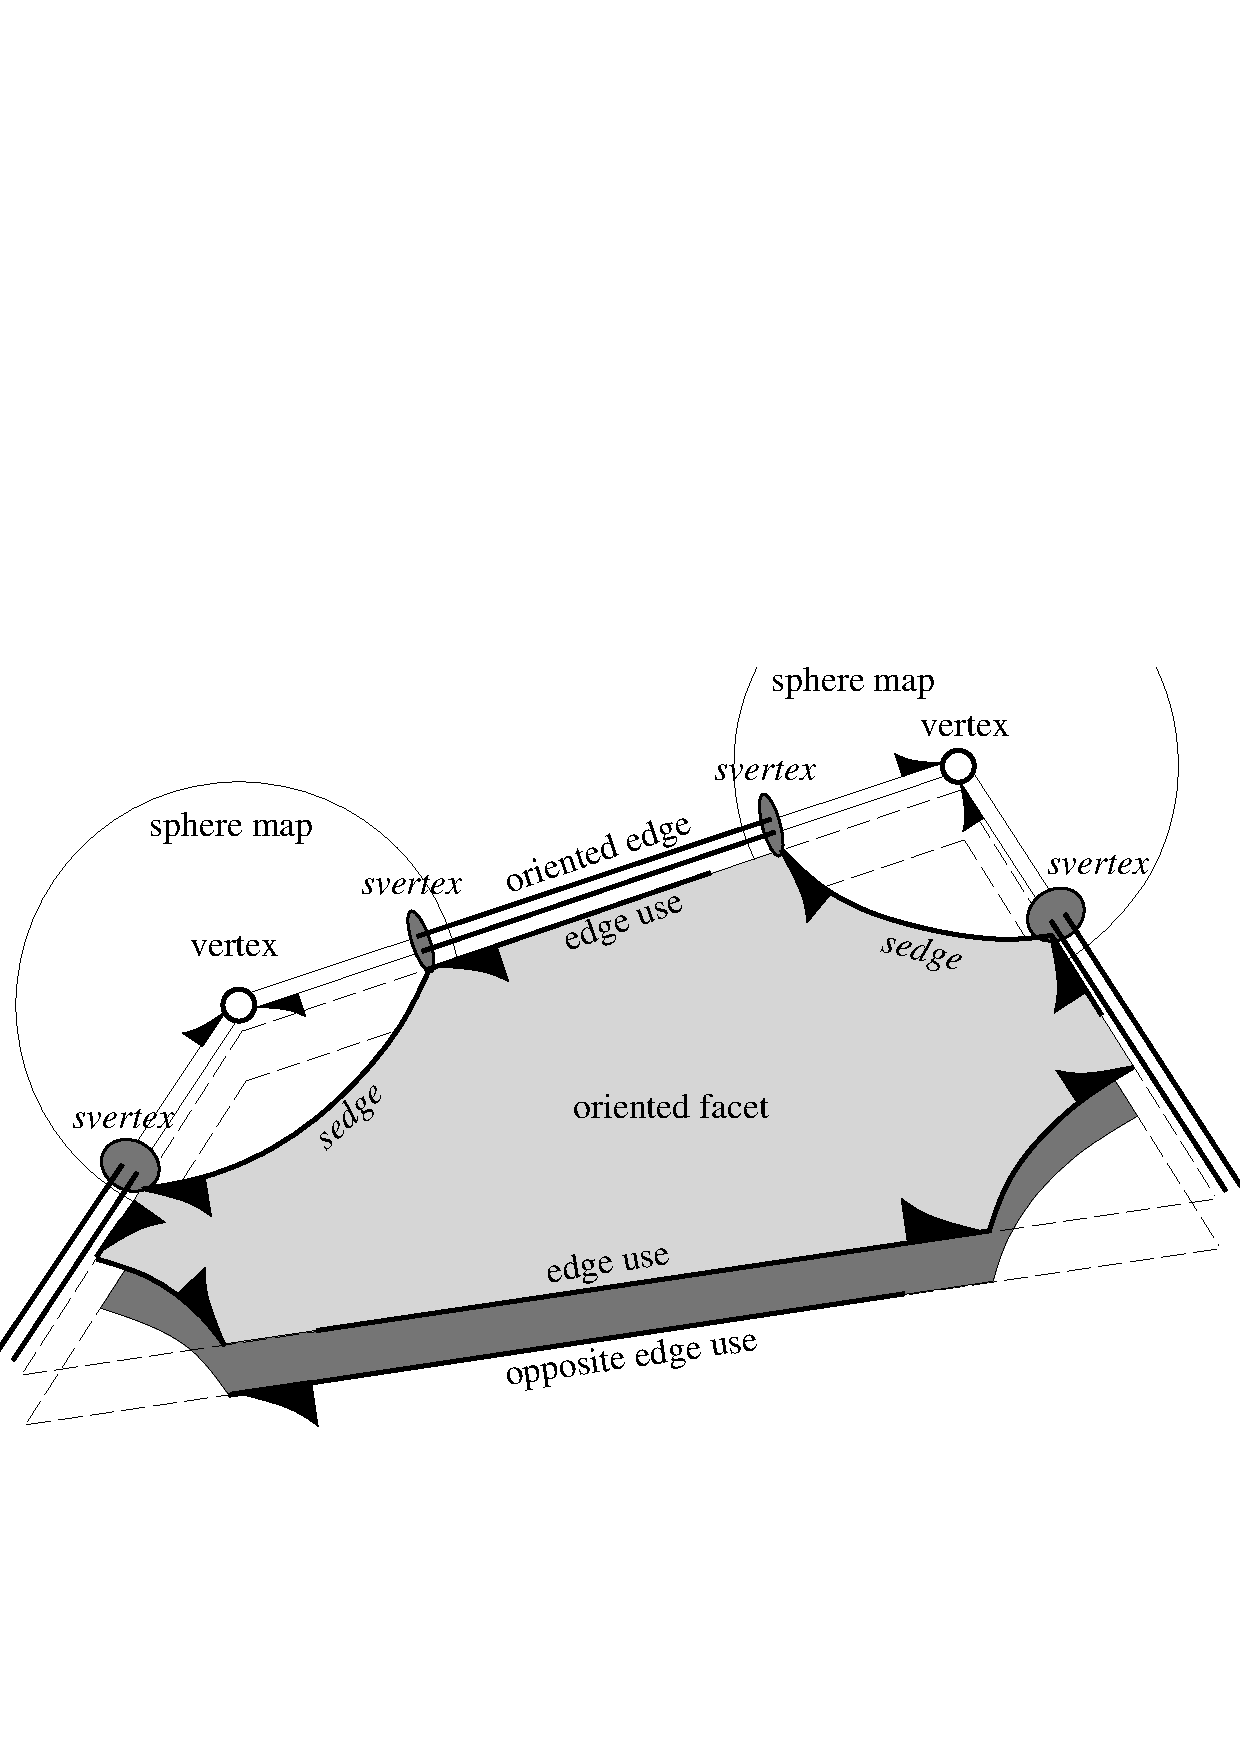
\includegraphics[width=0.6\textwidth]{Nef_3/fig/snc.ips}%
      }
    \end{center}
\end{ccTexOnly}

\begin{ccHtmlOnly}
    <CENTER>
        <img src="fig/snc.gif" alt="Steps in making a cube."><P>
    </CENTER>
\end{ccHtmlOnly}

We depart slightly from the
definition of faces in a Nef polyhedron; we represent the connected
components of a face individually and do not implement additional
bookkeeping to recover the original faces (e.g., all edges on a common
supporting line with the same local pyramid) as this is not needed in
our algorithms.  We discuss features in the increasing order of 
dimension.

\begin{description}
    \item[edges:] 
        We store two oppositely oriented edges for each edge
        and have a pointer from one oriented edge to its opposite edge.
        Such an oriented edge can be identified with an \emph{svertex}
        in a sphere map; it remains to link one \emph{svertex} with
        the corresponding opposite \emph{svertex} in the other sphere map.
    \item[edge uses:]
        An edge can have many incident facets (non-manifold situation).
        We introduce two oppositely oriented edge-uses for each incident
        facet; one for each orientation of the facet. An edge-use points 
        to its corresponding oriented edge and to its oriented facet.   
        We can identify an edge-use with an oriented \emph{sedge} in the 
        sphere map, or, in the special case also with an
        \emph{sloop}. Without mentioning it explicitly in the
        remainder, all references to \emph{sedge\/} can also refer to
        \emph{sloop}.
    \item[facets:]
        We store oriented facets as boundary cycles of oriented 
        edge-uses. We have a distinguished outer boundary cycle and 
        several (or maybe none) inner boundary cycles representing holes
        in the facet. Boundary cycles are linked in one direction. We can 
        access the other traversal direction when we switch to the oppositely
        oriented facet, i.e., by using the opposite edge-use.
    \item[shells:]
        The volume boundary decomposes into different connected
        components, the \emph{shells}. They consist of a connected set
        of facets, edges, and vertices incident to this volume. Facets 
        around an edge form a radial order that is captured in the
        radial order of \emph{sedges} around an \emph{svertex} in the
        sphere map. Using this information, we can trace a shell from
        one entry element with a graph search. We offer this graph
        traversal in a visitor design pattern to the user.
    \item[volumes:]
        A volume is defined by a set of shells, one outer shell containing
        the volume and several (or maybe none) inner shells separating voids
        which are excluded from the volume.
\end{description}

For each face we store a label, e.g., a set-selection mark, which
indicates whether the face is part of the solid or if it is
excluded. We call the resulting data structure \emph{Selective Nef
Complex}, \emph{SNC} for short~\cite{cgal:ghhkm-bosnc-03}. However, in
\cgal\ we identify the names and call the \emph{SNC} data structure
\ccc{CGAL::Nef_polyhedron_3}. 

% +------------------------------------------------------------------------+
\section{Infimaximal Box}
\label{sectionNef_3InfiBox}

We call a Nef polyhedron \emph{bounded} if its boundary is bounded,
i.e., finite, and \emph{unbounded} otherwise. Note that unbounded
point sets can have a bounded boundary, for example, the complement of
a cube has an unbounded outer volume, but its boundary remains bounded.

Using a boundary representation, it is convenient (conceptually and in
our implementation) to consider bounded Nef polyhedra only.  Bounded
Nef polyhedra are also closed under boolean set operations. However, one
needs to start with bounded primitives; the conceptually nice
halfspaces cannot be used. Instead, we offer a construction from oriented
2-manifolds represented in a  \ccc{CGAL::Polyhedron}, see
Section~\ref{subsectionNef_3Polyhedron} below.

In order to handle unbounded Nef polyhedra conceptually in the same
way as we handle bounded Nef polyhedra, we intersect them with a
bounding volume of size $[-R,R]^3$, where $R$ is a symbolical
unspecified value, which is finite but larger than all coordinate
values that may occur in the bounded part of the polyhedron. As a
result, each Nef polyhedron becomes bounded.  We call the boundary of
the bounding volume the \emph{infimaximal
  box}~\cite{cgal:sm-iftml-00}.

We clip lines and rays at the infimaximal box. The intersection points
with the infimaximal box are called \emph{non-standard points}, which
are points whose coordinates are $-R$ or $R$ in at least one
dimension, and linear functions $f(R)$ for the other dimensions. Such
extended points (and developed from there also extended segments etc)
are provided in \cgal\ with extended
kernels---\ccc{CGAL::Extended_cartesian} and
\ccc{CGAL::Extended_homogeneous}.  They are regular \cgal\ kernels
with a polynomial type as coordinate number type.

As long as an extended kernel is used, the full functionality provided
by the \ccc{CGAL::Nef_polyhedron_3} class is available. If kernel that 
does not use polynomial to represent coordinates is used, it is not 
possible to create or load unbounded Nef
polyhedra, but all other operations work as expected. We provided both
possibilities, since the restriction to bounded Nef polyhedra improves
considerably space requirements (plain number type instead of
polynomial), and runtime performance.


% +========================================================================+%
\section{Regularized Set Operations}
% +========================================================================+

Since manifolds are not closed under boolean operations, Requicha
proposes to use \emph{regularized set operations}~\cite{cgal:km-st-76,
  cgal:r-rrstm-80}.  A set is \emph{regular}, if it equals the closure
of its interior. A regularized set operation is defined as the 
standard set operation followed by a regularization of the result.
Regularized sets are closed under regularized set operations.

Regularized set operations are important since they simplify the class
of solids to exclude lower dimensional features and the boundary
belongs to the point set. These properties are considered to reflect
the nature of physical solids more closely.

Regularized polyhedral sets are a subclass of Nef polyhedra. We provide the
\ccc{regularization} operation as a shortcut for the consecutive execution
of the \ccc{interior} and the \ccc{closure} operations.

% +========================================================================+
\section{Example Programs}
% +========================================================================+

The following example gives a first impression of how to instantiate
and use \ccc{Nef_polyhedron_3}. We use the \ccc{CGAL::Cartesian}
kernel.  All Cartesian and homogeneous kernels of \cgal\ are suitable
if the number type parameter follows the usual requirements of being a
model of the \ccc{CGAL::FieldNumberType} concept for the Cartesian
kernels, or the \ccc{CGAL::RingNumberType} concept for the homogeneous
kernels, respectively. Note however, that in the current state, the
Nef polyhedron works only with \cgal\ kernels. The implementation
makes use of \cgal\ specific functions in kernel objects, and does not
yet offer a designed interface to a clean kernel concept that could be
offered by an external kernel as well.

The example creates two Nef polyhedra---\ccc{N0} is the empty set,
while \ccc{N1} represents the full space, i.e., the set of all points
in the 3-dimensional space. The assertion assures that the empty set
is the complement of the full space.

\ccIncludeExampleCode{Nef_3/simple.C}

% +------------------------------------------------------------------------+
\subsection{Construction and Comparison}

This example shows the various constructors. We can create the empty
set, which is also the default constructor, and the full space, i.e.
all points of $\mathbb{R}^3$ belong to the polyhedron. We can create a
halfspace defined by a plane bounding it. It is only available if an
extended kernel is used. The halfspace constructor has a second
parameter that specifies whether the defining plane belongs to the
point set (\ccc{Nef_polyhedron::INCLUDED}) or not
(\ccc{Nef_polyhedron::EXCLUDED}). The default value is
\ccc{Nef_polyhedron::INCLUDED}. Additionally, we can create a
\ccc{Nef_polyhedron_3} from a \ccc{Polyhedron_3}, see the Section
\ref{subsectionNef_3Polyhedron} below.

We can compute the point sets of two Nef polyhedra for equality and
proper subset relationships. We offer the usual comparison operators
\ccc{==}, \ccc{!=}, \ccc{<=}, \ccc{>=}, \ccc{<} and \ccc{>}. 

Nef polyhedra have the important feature that a representation that is
called the \emph{reduced W\"urzburg structure} is unique, i.e., two
point sets of Nef polyhedra are equal if and only if the
representations are equal. The proof for the reduced W\"urzburg
structure carries over to our representation and the comparison
operators are therefore trivial to implement.

\ccIncludeExampleCode{Nef_3/construction.C}

% +------------------------------------------------------------------------+
\subsection{Point Set Operations}

As explained in the introduction, Nef polyhedra are closed under all
boolean set operations. The class \ccc{Nef_polyhedron_3} provides
functions and operators for the most common ones: complement
(\ccc{operator!}), union (\ccc{operator+}), difference
(\ccc{operator-}), intersection (\ccc{operator*}) and symmetric
difference (\ccc{operator^}). Additionally, the operators \ccc{*=},
\ccc{-=}, \ccc{*=} and \ccc{^=} are defined.

\ccc{Nef_polyhedron_3} also provides the topological operations
\ccc{interior()}, \ccc{closure()} and \ccc{boundary()}. With
\ccc{interior()} one deselects all boundary items, with
\ccc{boundary()} one deselects all volumes, and with \ccc{closure()}
one selects all boundary items.

\ccIncludeExampleCode{Nef_3/point_set_operations.C}

% +------------------------------------------------------------------------+
\subsection{Transformation}

Using the \ccc{std::transform} function, a Nef polyhedron can be translated, 
rotated and scaled. The usage is shown in the following example:

\ccIncludeExampleCode{Nef_3/transformation.C}

% +------------------------------------------------------------------------+
\subsection{The Interface between \ccc{Polyhedron_3} and 
    \ccc{Nef_polyhedron_3}}
\label{sectionNef_3Polyhedron}

\ccc{Nef_polyhedron_3} provides an interface for the conversion between
polyhedral surfaces represented with the \ccc{CGAL::Polyhedron_3} class
and \ccc{Nef_polyhedron_3}.  \ccc{Polyhedron_3} represents orientable
2-manifold objects with boundaries. However, we exclude surfaces with
boundaries from the conversion to \ccc{Nef_polyhedron_3} since they
have no properly defined volume.

Both conversion directions can only be performed if the boundary of
the point set is an oriented closed 2-manifold.
\ccc{Nef_polyhedron_3} provides the function \ccc{is_simple()} and
\ccc{Polyhedron_3} provides the function \ccc{is_closed()} to test for
this property. The usage is illustrated by the example program below.

The conversion gives us the possibility to use several file formats.
\ccc{Polyhedron_3} can read the ({\tt .off}) file format and can write
the ({\tt .off}), OpenInventor ({\tt .iv}), VRML 1.0 and 2.0 ({\tt
  .wrl}) and Wavefront Advanced Visualizer object format ({\tt .obj}),
see Section~\ref{sectionPolyIO}.

\ccIncludeExampleCode{Nef_3/interface_polyhedron.C}

% +------------------------------------------------------------------------+
\subsection{Using an Extended Kernel}

The provided extended kernels are used the same way as any other
\cgal\ kernel.  The essential difference is, that coordinates are not
represented by the number type that was used to parameterize the
kernel type, but by a \ccc{Nef_polynomial} parametrized by that number
type.

The example iterates all vertices of a given Nef polyhedron and decides whether
it is an standard vertex or a vertex on the infimaximal box. Furthermore, it 
tests whether any of the vertices is at $(R,R,R)$. Recall that $R$ was
the symbolical value, large but finite, for the size of the infimaximal box. 

\ccIncludeExampleCode{Nef_3/extended_kernel.C}

% +========================================================================+
\section{File I/O}
% +========================================================================+
\label{sectionNef_3IO}

\ccc{Nef_polyhedron_3} provides an input and an output operator for a
proprietary file format. It includes the complete incidence structure,
the geometric data, and the marks of each item.  The output depends on
the output operators of the geometric primitives provided by the
traits class, and on the output operators of the used number type.
Therefore, it is necessary to use the same kernel and the same number
type for input and output operations.

We recommend to use the \cgal\ kernels \ccc{Homogeneous},
\ccc{Simple_homogeneous}, or \ccc{Extended_homogeneous}. We provide
compatibility between the input and output of these kernels.
Especially, it is possible to write a bounded Nef polyhedron using the
\ccc{Extended_homogeneous} kernel and to read it afterwards using one
of the two others.

Using \cgal\ stream modifiers the following output formats can be chosen: 
ASCII(\ccc{set_ascii_mode}), binary(\ccc{set_binary_mode}) or 
pretty(\ccc{set_pretty_mode}). The mandatory format is the ASCII format.

\ccIncludeExampleCode{Nef_3/nefIO.C}

% +========================================================================+
\section{Further Example Programs}
% +========================================================================+

% +------------------------------------------------------------------------+
\subsection{Exploring a Sphere Map}

A sphere map is explored by using the function \ccc{get_sphere_map}, which 
returns the sphere map of the specified vertex as a \ccc{Nef_polyhedron_S2}.
\ccc{Nef_polyhedron_S2} provides the functionality necessary for the
exploration.
Note, that one has to use
the type \ccc{Nef_polyhedron_S2} as specified in \ccc{Nef_polyhedron_3} as 
is shown in the following example.

\ccIncludeExampleCode{Nef_3/exploration_SM.C}

% +------------------------------------------------------------------------+
\subsection{Exploring Shells}

A \emph{shell} of a Nef polyhedron is the connected part of the
surface incident to a certain volume.  Each halffacet, sface and
shalfedge belongs to a single shell. The figure below illustrates the
notion of a shell.  It shows a Nef polyhedron with two volumes and
three shells.

\begin{ccTexOnly}
    \begin{center}
      \parbox{0.4\textwidth}{%
          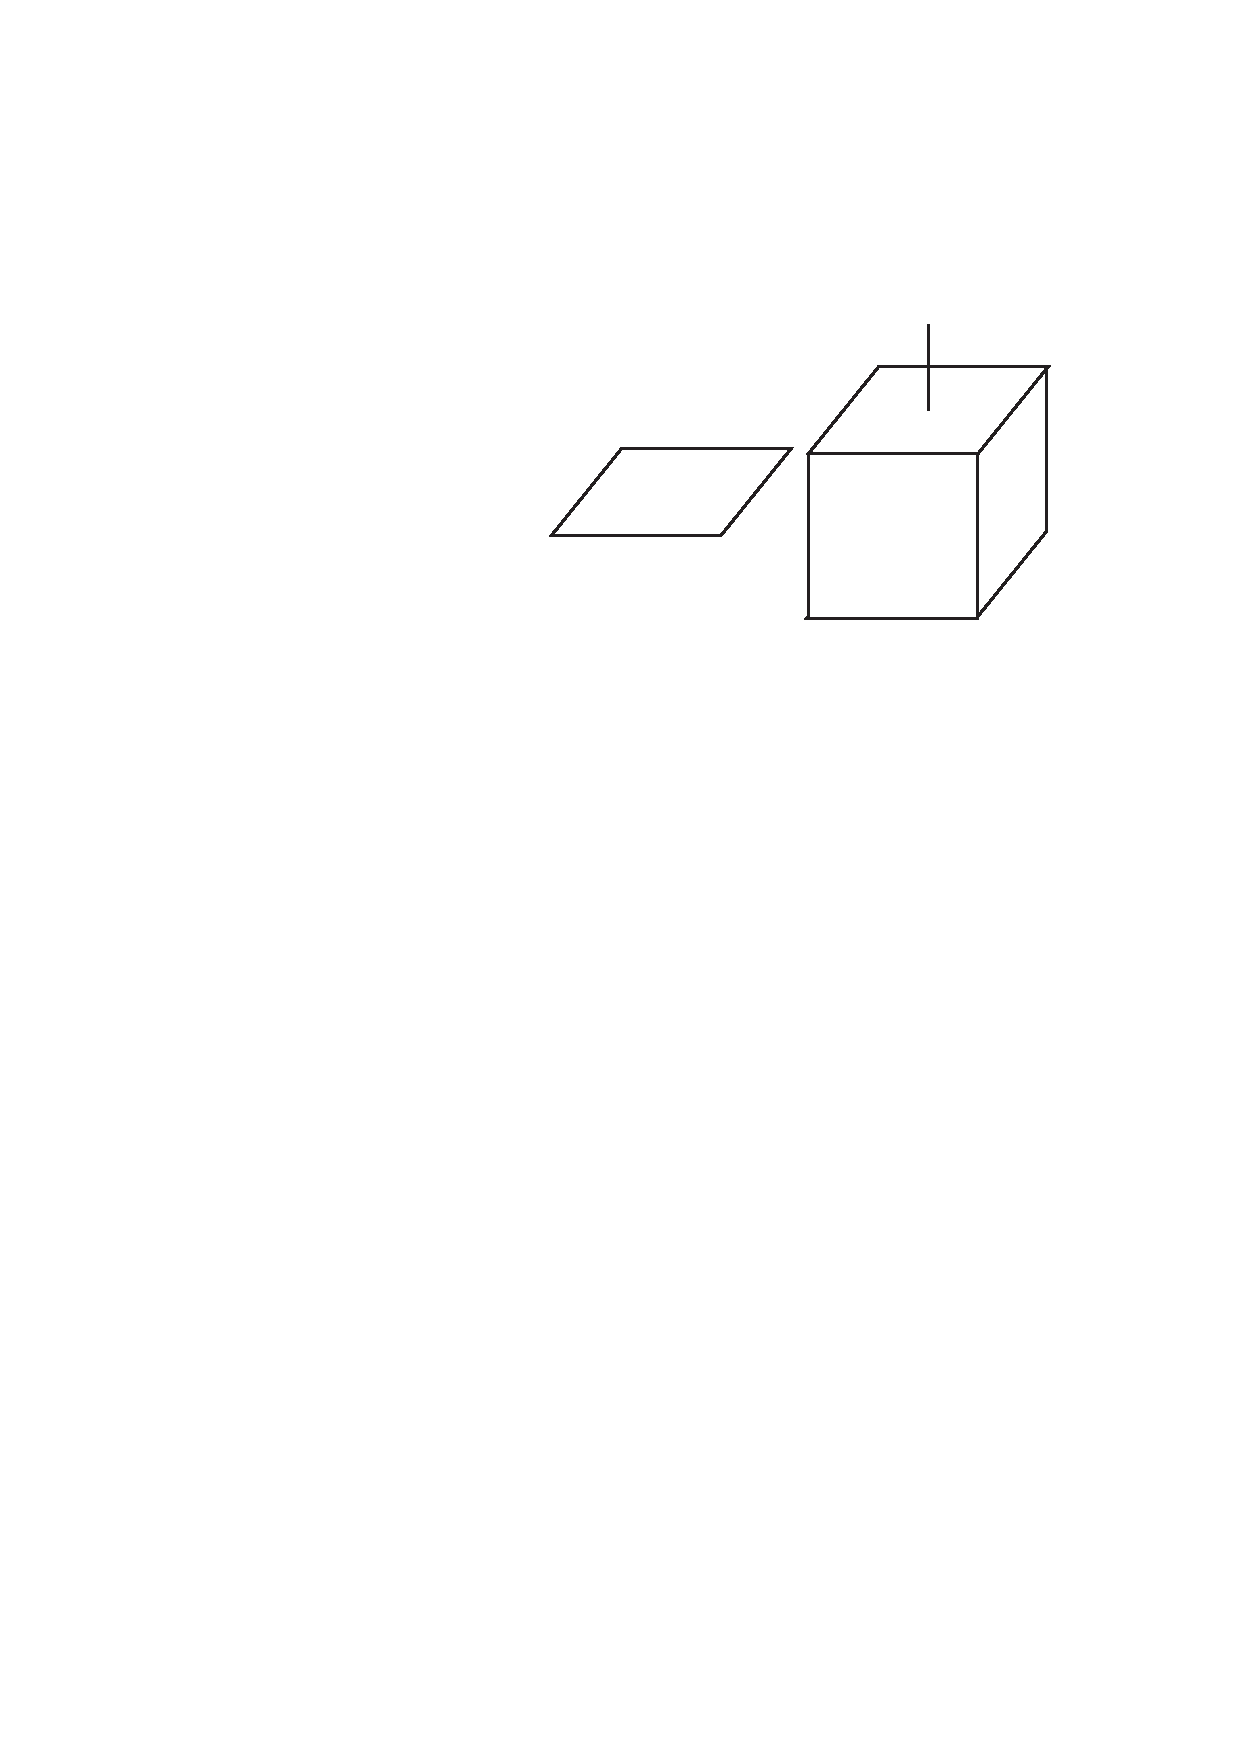
\includegraphics[width=0.4\textwidth]{Nef_3/fig/shells}%
      }
    \end{center}
\end{ccTexOnly}

\begin{ccHtmlOnly}
    <CENTER>
        <img src="fig/shells.gif" alt="Steps in making a cube."><P>
    </CENTER>
\end{ccHtmlOnly}


The first volume is the outer volume and the second volume is the
interior of the cube. The first shell is the whole surface of the left
object. The second shell is the outer surface of the right object, and
the third shell is the inner surface of the right object. 

In detail, the first shell consists of two halffacets, eight halfedges
and four vertices. The second shell consists of the eight vertices of
the cube plus the two endpoints of the antenna, all halffacets
oriented outwards, and all halfedges. The third shell consists of the
same eight vertices of the cube, plus the endpoint of the antenna
that is in contact with the cube, all halffacets
oriented inwards, and all halfedges (the same as for the second shell).

\begin{ccTexOnly}
    \begin{center}
      \parbox{0.4\textwidth}{%
          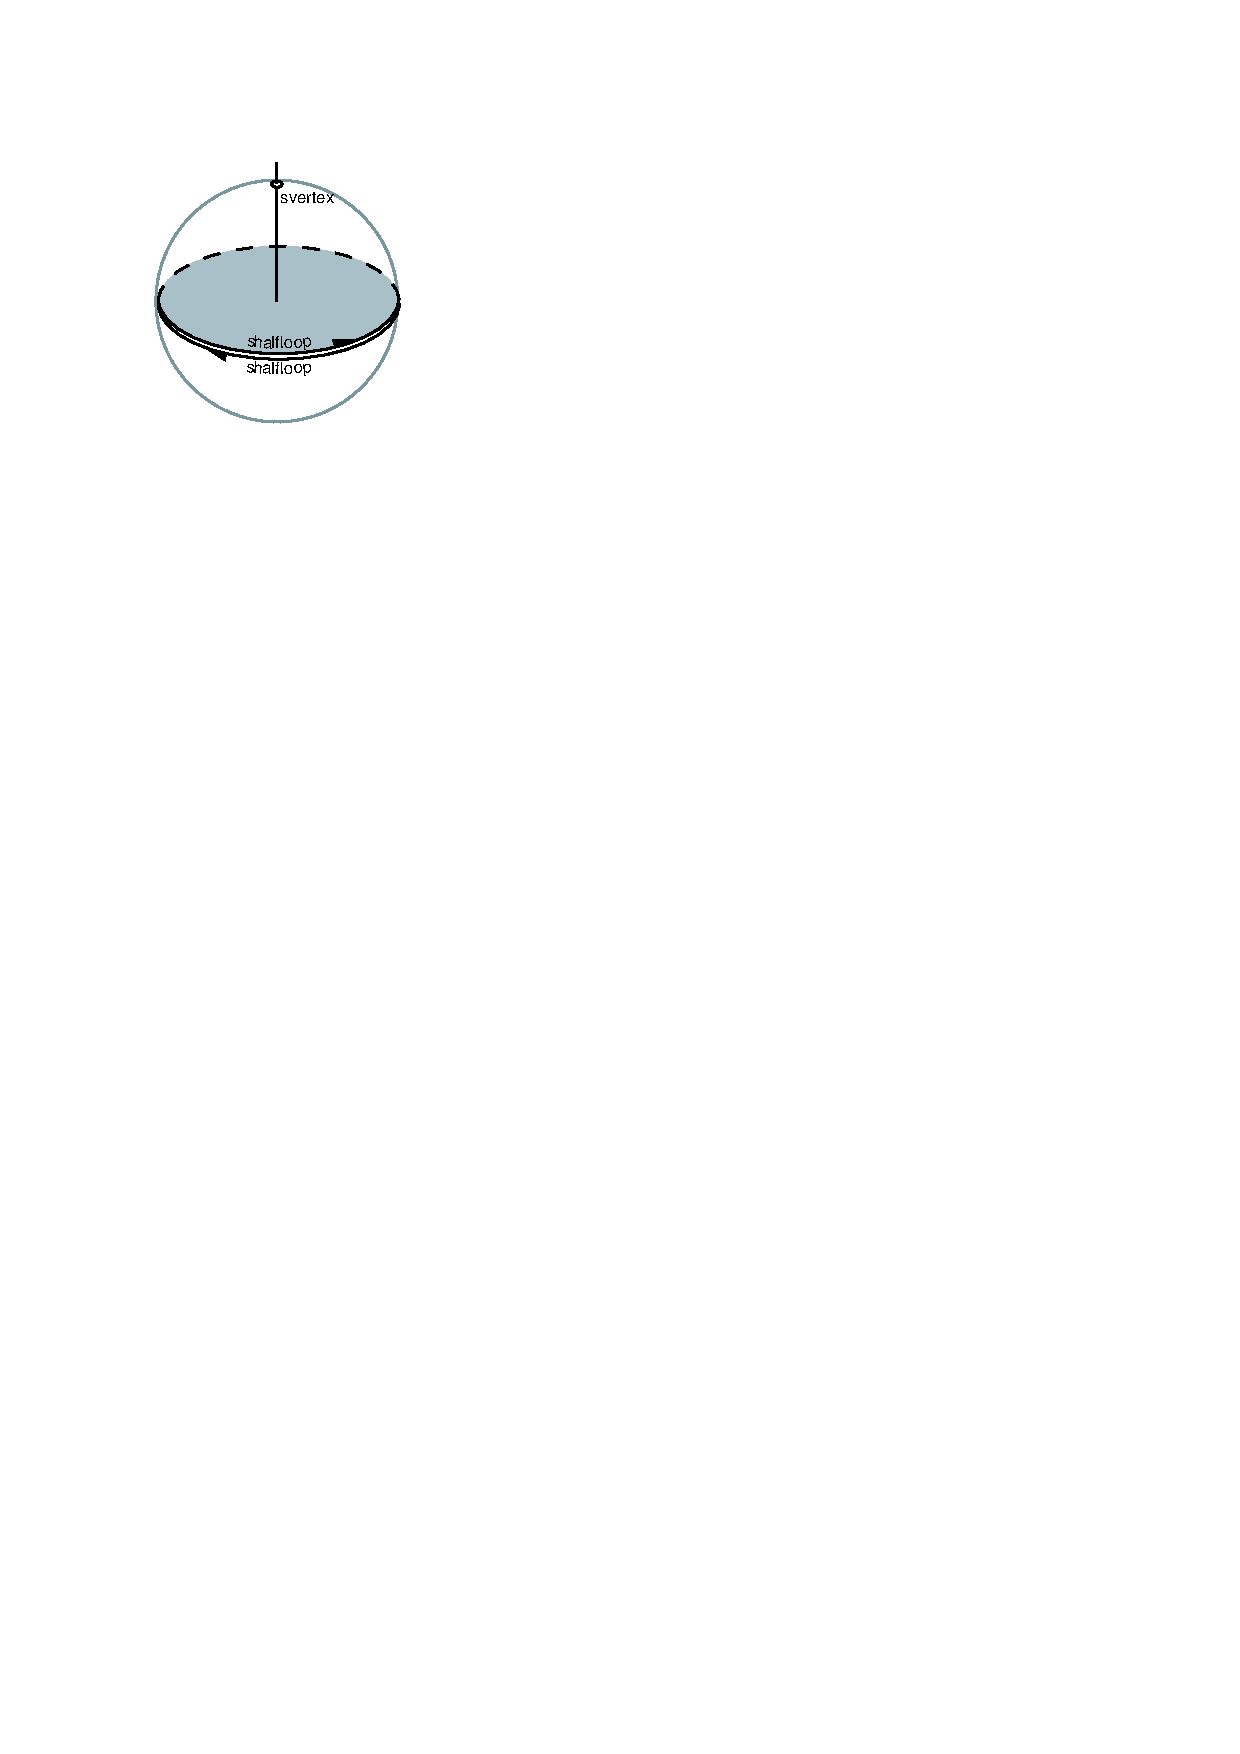
\includegraphics[width=0.4\textwidth]{Nef_3/fig/closeup}%
      }
    \end{center}
\end{ccTexOnly}

\begin{ccHtmlOnly}
    <CENTER>
        <img src="fig/closeup.gif" alt="Steps in making a cube."><P>
    </CENTER>
\end{ccHtmlOnly}

We discuss how sfaces, shalfedges, and sloops belong to the shells
with a closeup view of the situation at the antenna foot. As you can
see, there are three items on the sphere map - a shalfloop for each
halffacet which intersects the sphere, and an svertex where the
antenna intersects the sphere. The upper shalfloop lies on the 
halffacet which is oriented outwards and is therefore also 
oriented outwards. This shalfloop and the svertex belong to the
second shell.
The other shalfloop lies on the inwards oriented halffacet and is 
oriented inwards, too. This shalfloop belongs to the third shell. 

\ccc{Nef_polyhedron_3} offers a visitor interface to explore a shell
following the well-known visitor pattern~\cite{cgal:ghjv-dpero-95}.
The interface is illustrated by the following example.

\ccIncludeExampleCode{Nef_3/shell_exploration.C}

The function \ccc{visit_shell_objects(SFace_const_handle sf, Visitor&
  V)} explores a shell starting at the \ccc{sf}. The second argument
expects any class providing the (possibly empty) functions
\ccc{visit(Vertex_const_handle)}, \ccc{visit(Halfedge_const_handle)}
(remember that Halfedge is the same type as SVertex),
\ccc{visit(Halffacet_const_handle)},
\ccc{visit(SHalfedge_const_handle)},
\ccc{visit(SHalfloop_const_handle)} and
\ccc{visit(SFace_const_handle)}.  The \ccc{visit_shell_objects}
function will call \ccc{visit} for each item belonging to the shell
once. There are no further requirements on that class.

In the example, the class \ccc{Shell_explorer} is passed as second argument
to \ccc{visit_shell_objects}. Its task is to find the lexicographically
smallest vertex of a shell. Its internal state consists of three variables. 
The first one is a reference to the explored Nef polyhedron. This reference
is often necessary to retrieve information from the Nef polyhedron. The
second variable \ccc{v_min} stores the smallest vertex found so far, and
the third variable \ccc{first} is initialized to \ccc{false} to signal that no
vertex has been visited so far. After the first vertex has been visited 
\ccc{first} is changed to \ccc{true}.

\ccc{Shell_explorer} provides further member functions. After the
exploration of a shell the \ccc{minimal_vertex} function retrieves the
smallest vertex. The \ccc{reset_minimal_vertex} function allows one to
use the same instance of \ccc{Shell_explorer} on multiple shells. In
this case, the \ccc{reset_minimal_vertex} function has to be called
between the exploration of two shells.

The example program uses the \ccc{Shell_explorer} for each shell of
the given Nef polyhedron once and reports the smallest vertex of each
shell to the standard output.

% +------------------------------------------------------------------------+
\subsection{Point Location}

The \ccc{locate(Point_3 p)} function locates the point \ccc{p} in the
Nef polyhedron and returns the item the point belongs to. The
\ccc{locate} function returns an instance of \ccc{Object_handle},
which is a polymorphic handle type representing any handle type, no
matter if it is mutable or const.  For further usage of the result,
the \ccc{Object_handle} has to be casted to the concrete handle type.
The \ccc{CGAL::assign} function performs such a cast. It returns a
boolean that reports the success or the failure of of the cast.
Looking at the possible return values of the \ccc{locate} function,
the \ccc{Object_handle} can represent a \ccc{Vertex_const_handle}, a
\ccc{Halfedge_const_handle}, a \ccc{Halffacet_handle}, or a
\ccc{Volume_const_handle}. One of the four casts will succeed.

\ccIncludeExampleCode{Nef_3/point_location.C}

% +------------------------------------------------------------------------+
\subsection{Visualizing a 3D Nef polyhedron}

With the \ccc{Nef_Visualizor_OpenGL_3} class an interface to OpenGL
visualization is offered, however, it is intended for debugging and a
first simple illustration. In particular, the GUI is fixed and not
extensible. The \ccc{Nef_Visualizor_OpenGL_3} class offers a
constructor from a Nef polyhedron, a \ccc{draw} function  which
determines the state in which the Nef polyhedron is shown, and the
\ccc{CGAL::OGL::start_viewer()}  function which opens the visualizor
window and starts the event processing for the interactive control
available in the viewer. The \ccc{CGAL::OGL::start_viewer()}  function
never returns and the application must be terminated with the proper
entry in the pop-up menu of the visualizer. The viewer is easy to use
as can be seen in the following example.

\begin{ccTexOnly}
    \begin{center}
      \parbox{0.4\textwidth}{%
          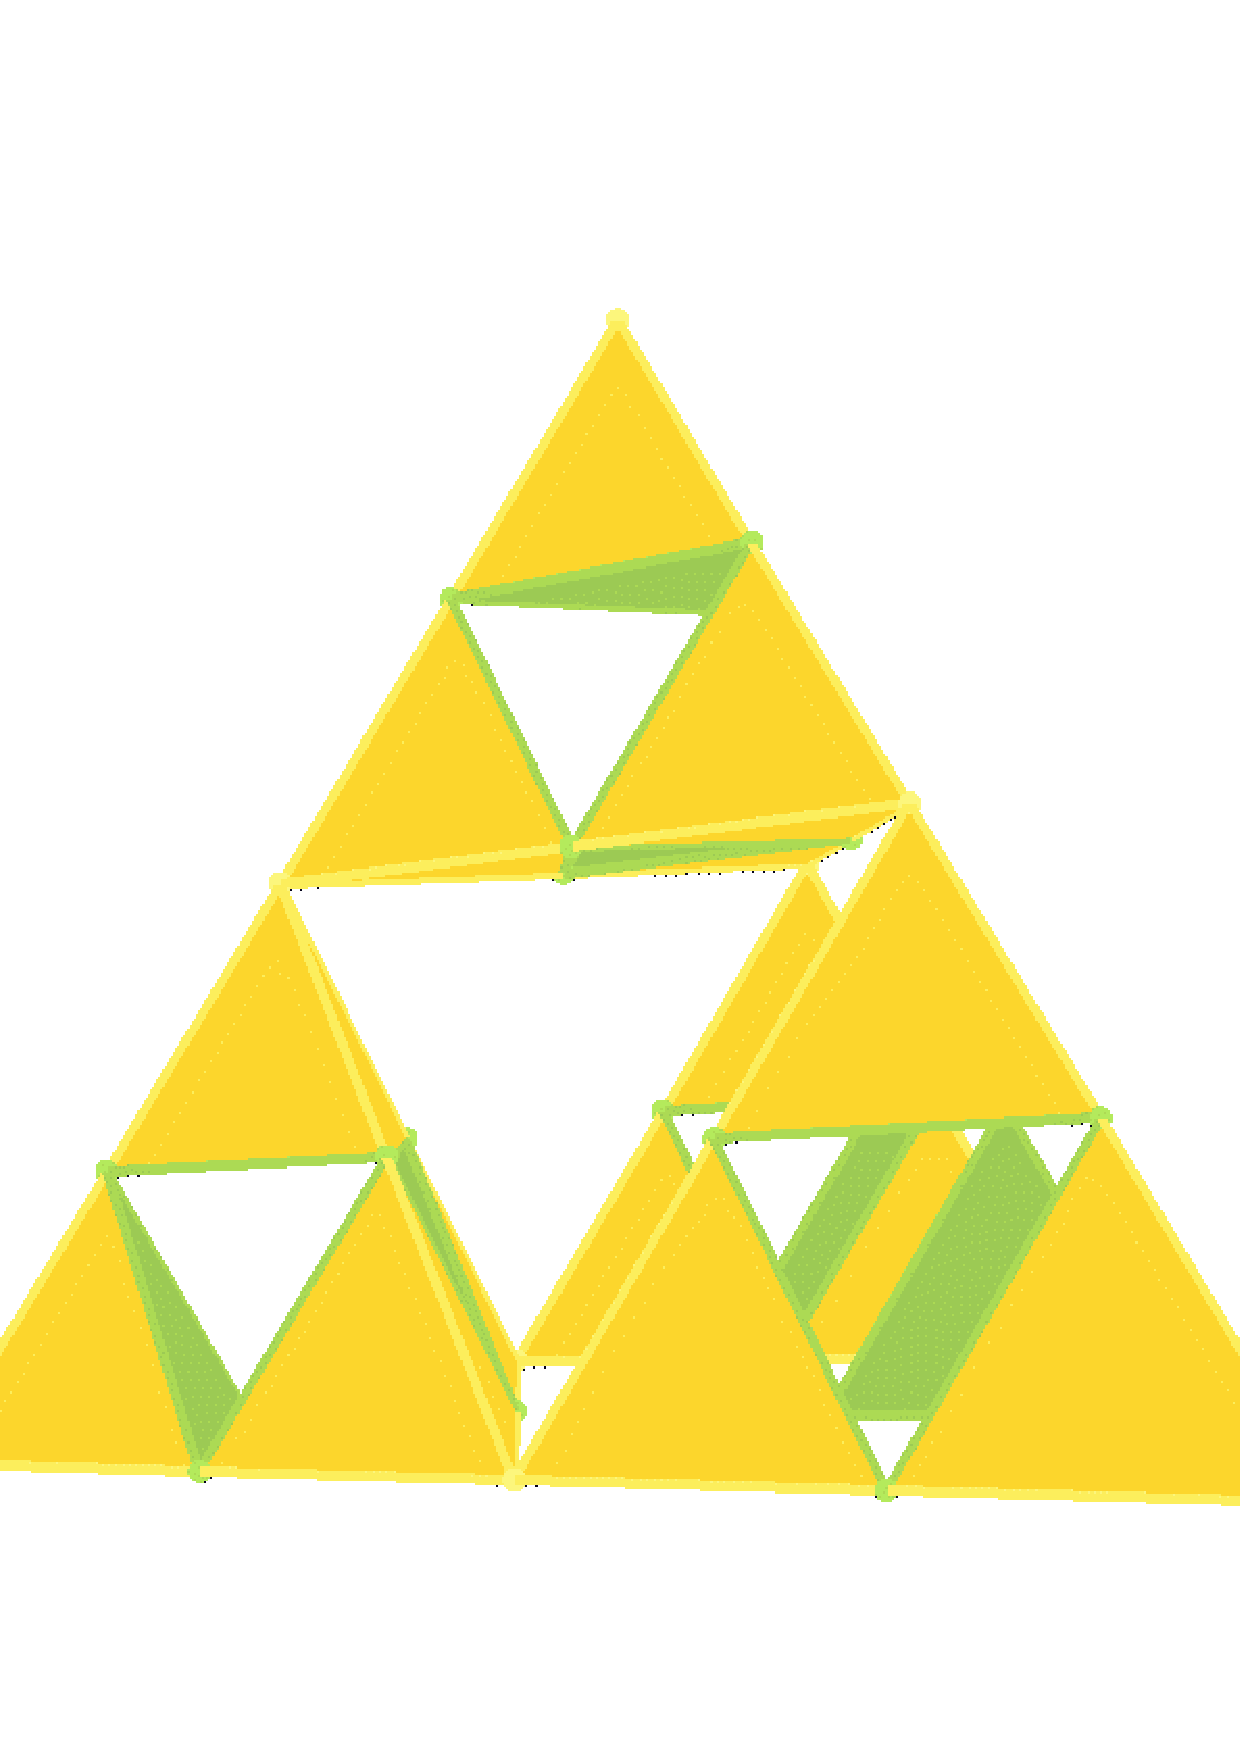
\includegraphics[width=0.4\textwidth]{Nef_3/fig/visualization_SNC}%
      }
    \end{center}
\end{ccTexOnly}

\begin{ccHtmlOnly}
    <CENTER>
       <img src="./fig/visualization_SNC.png" alt="Steps in making a cube."><P>
    </CENTER>
\end{ccHtmlOnly}

\ccIncludeExampleCode{Nef_3/visualization_SNC.C}

% +------------------------------------------------------------------------+
\subsection{Visualizing a Sphere Map}

A sphere map can be visualized using the interface between
\ccc{Nef_polyhedron_S2} and \ccc{Nef_polyhedron_3}.

\ccIncludeExampleCode{Nef_3/visualization_SM.C}

%% EOF %%
